\chapter{Route Acquisition and Terrain Data Pipeline}
\label{ch:routes}

\Cref{sec:input_definitions} defined the route profile $\route$ as a piecewise field of grade, curvature, and speed limit sampled along a track. \Cref{ch:refsim} then treats that field as an input it is simply handed. This chapter explains where that input actually comes from.

One of the locked decisions behind this thesis is that routes are built from real terrain rather than invented from scratch (\cref{sec:input_definitions}). The reasoning is straightforward: a surrogate model is only as convincing as the data it is trained on, and a grade profile that looks nothing like a real railway line is a weak foundation for later claims about generalization. Satisfying that decision, however, is not a small task. It requires pulling raw track geometry from an open mapping database, turning that geometry into clean, continuous corridors, attaching real elevation data to it, and converting the result into the exact numerical fields the simulator and surrogate expect. This chapter documents the pipeline that does that.

The pipeline is organized as four stages plus an export step, each with its own storage folder and its own tab in an accompanying application:
\begin{equation*}
    \text{acquire} \rightarrow \text{resample} \rightarrow \text{elevation} \rightarrow \text{profile} \rightarrow \text{export}
\end{equation*}
It is built to run in batches: a route is fetched and checked, good routes are collected, and a dataset is generated for that batch, rather than attempting to process an entire national rail network in one pass.

Five corridors were acquired this way, and the datasets used later in the thesis are built on them. One of the five was later rejected. Its raw elevation turned out to be wrong before any processing was applied, and \cref{sec:route_raw_qa} describes the check that now catches this kind of failure. The last part of the chapter (\cref{sec:route_scaling}) describes the attempt to scale acquisition beyond a handful of corridors, why the original crawl failed at that scale, and the national rail network dataset that replaced it.

\begin{figure}[h]
\centering
\caption{Overview of the route acquisition pipeline, from raw OpenStreetMap track data to the route-tensor fields consumed by the reference simulator.}
\label{fig:route_pipeline_overview}
\end{figure}

\section{Stage 1: Acquisition}
\label{sec:route_acquisition_stage1}

\subsection{Why acquisition has to be area-first}

Railway lines are not tidy, self-contained objects in OpenStreetMap (OSM) \cite{osm}. Track is mapped as many short, disconnected segments called ways, and while OSM does define route relations that are supposed to group these ways into a single named line, coverage for United States freight corridors is incomplete and a given relation does not reliably correspond to one clean, walkable corridor. Waiting for well-formed relations to exist would leave large parts of the network unusable.

\begin{figure}[htbp]
    \centering
    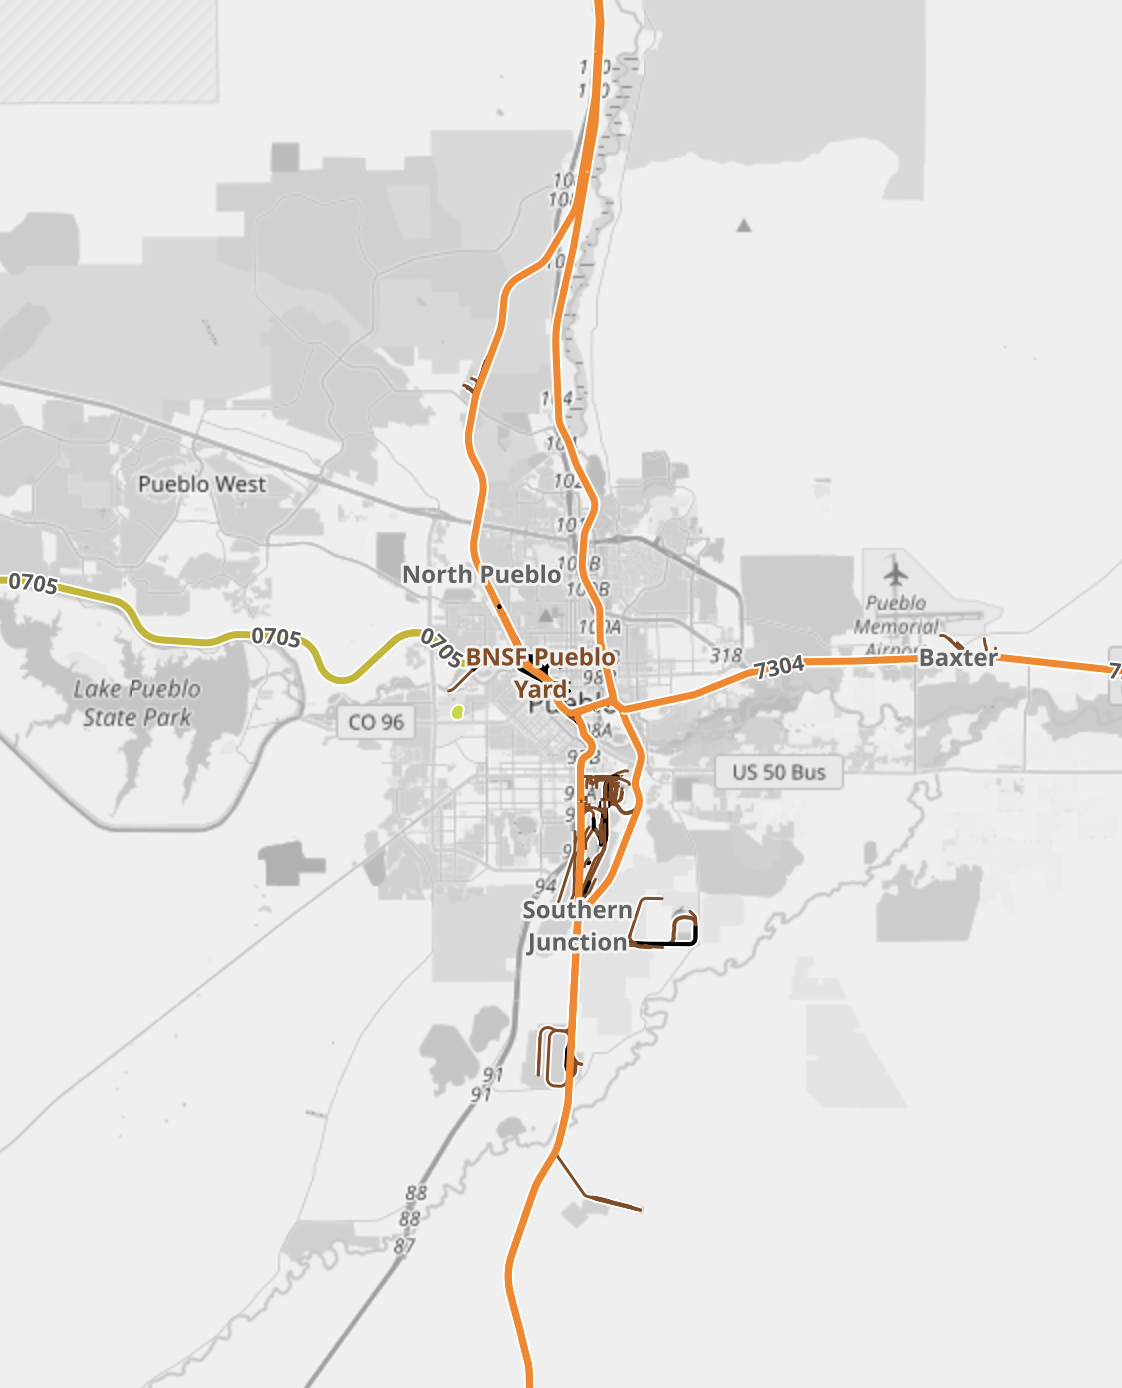
\includegraphics[width=0.62\textwidth]{thesis_imgs_7_15/route_generator/ORM_base.png}
    \caption{Railway mapping around Pueblo, Colorado, rendered from OpenStreetMap track data. Mainline corridors (orange) run through a dense tangle of yard and service track (brown) and meet at several junctions. There is no single map object corresponding to ``the line through Pueblo''; corridors have to be recovered from the segments.}
    \label{fig:route_orm_base}
\end{figure}

The pipeline therefore treats selection as area-first. A user specifies a bounding box or a radius around a point, all track ways inside that area are pulled, and the resulting tangle of segments is split back into corridors algorithmically rather than relying on OSM's own grouping. Fetching by relation ID is kept as a secondary path for the cases where a good relation happens to exist.

\subsection{Corridor extraction as a graph problem}

Once an area's track ways are pulled, they are assembled into a graph whose vertices are the endpoints and junctions of the track and whose edges are the individual way segments. Every vertex falls into one of three roles: a \emph{continuation} node has degree two and simply passes a line through; a \emph{line-end} has degree one and marks where a piece of track terminates; a \emph{junction} has degree three or higher and marks a real branch point. Corridors are then extracted as maximal paths through continuation nodes, breaking wherever a line-end or a junction is reached. This is what turns an unordered pile of map fragments into a set of distinct, traceable lines.

For the radius-based query mode, an optional bounded outward crawl extends this further: starting from the area first pulled, the pipeline follows each line's open ends past the edge of the original radius, issuing additional queries just beyond them, until each line reaches a natural end or a hard cap on distance, iteration count, or total ways is hit. This captures lines that only pass through the queried area rather than starting or ending inside it, while the cap keeps the crawl from expanding into the fully connected national network.

\subsection{Putting fragments back together}

OSM splits a single physical rail line into many ways wherever a junction, a bridge, or a change in tagging occurs, and sidings introduce additional junctions that fragment a line even further. A long corridor can therefore arrive as dozens of disconnected pieces. A grouping step re-links collinear fragments, across both real junctions and small unshared endpoint gaps, using endpoint proximity together with heading continuity (whether the fragments point the same direction where they meet). Nothing is merged or discarded in this step; fragments keep their identity and remain reversible, they are simply labeled with a shared line identifier and an order along that line, so later stages can stitch them into one ordered polyline. Ways tagged as sidings, spurs, yards, or crossovers are flagged as service track and kept out of this mainline grouping, though they can still be included in a batch if a user specifically wants them.

A related routine builds a robust centerline directly from a set of member ways, whether those ways come from a relation fetch or from a grouped corridor. It stitches unordered and reversed ways into one ordered polyline using shared endpoint nodes, with a coordinate-based fallback when node identifiers do not line up, and it explicitly detects gaps (gaps in space) and branches (points where more than one continuation is possible) rather than silently picking one. Duplicate junction vertices are removed, per-vertex tags such as speed limit, bridge, tunnel, cutting, and embankment are carried along, and geodesic arc length is computed for the whole line.

\subsection{Interactive selection}

\begin{figure}[htbp]
    \centering
    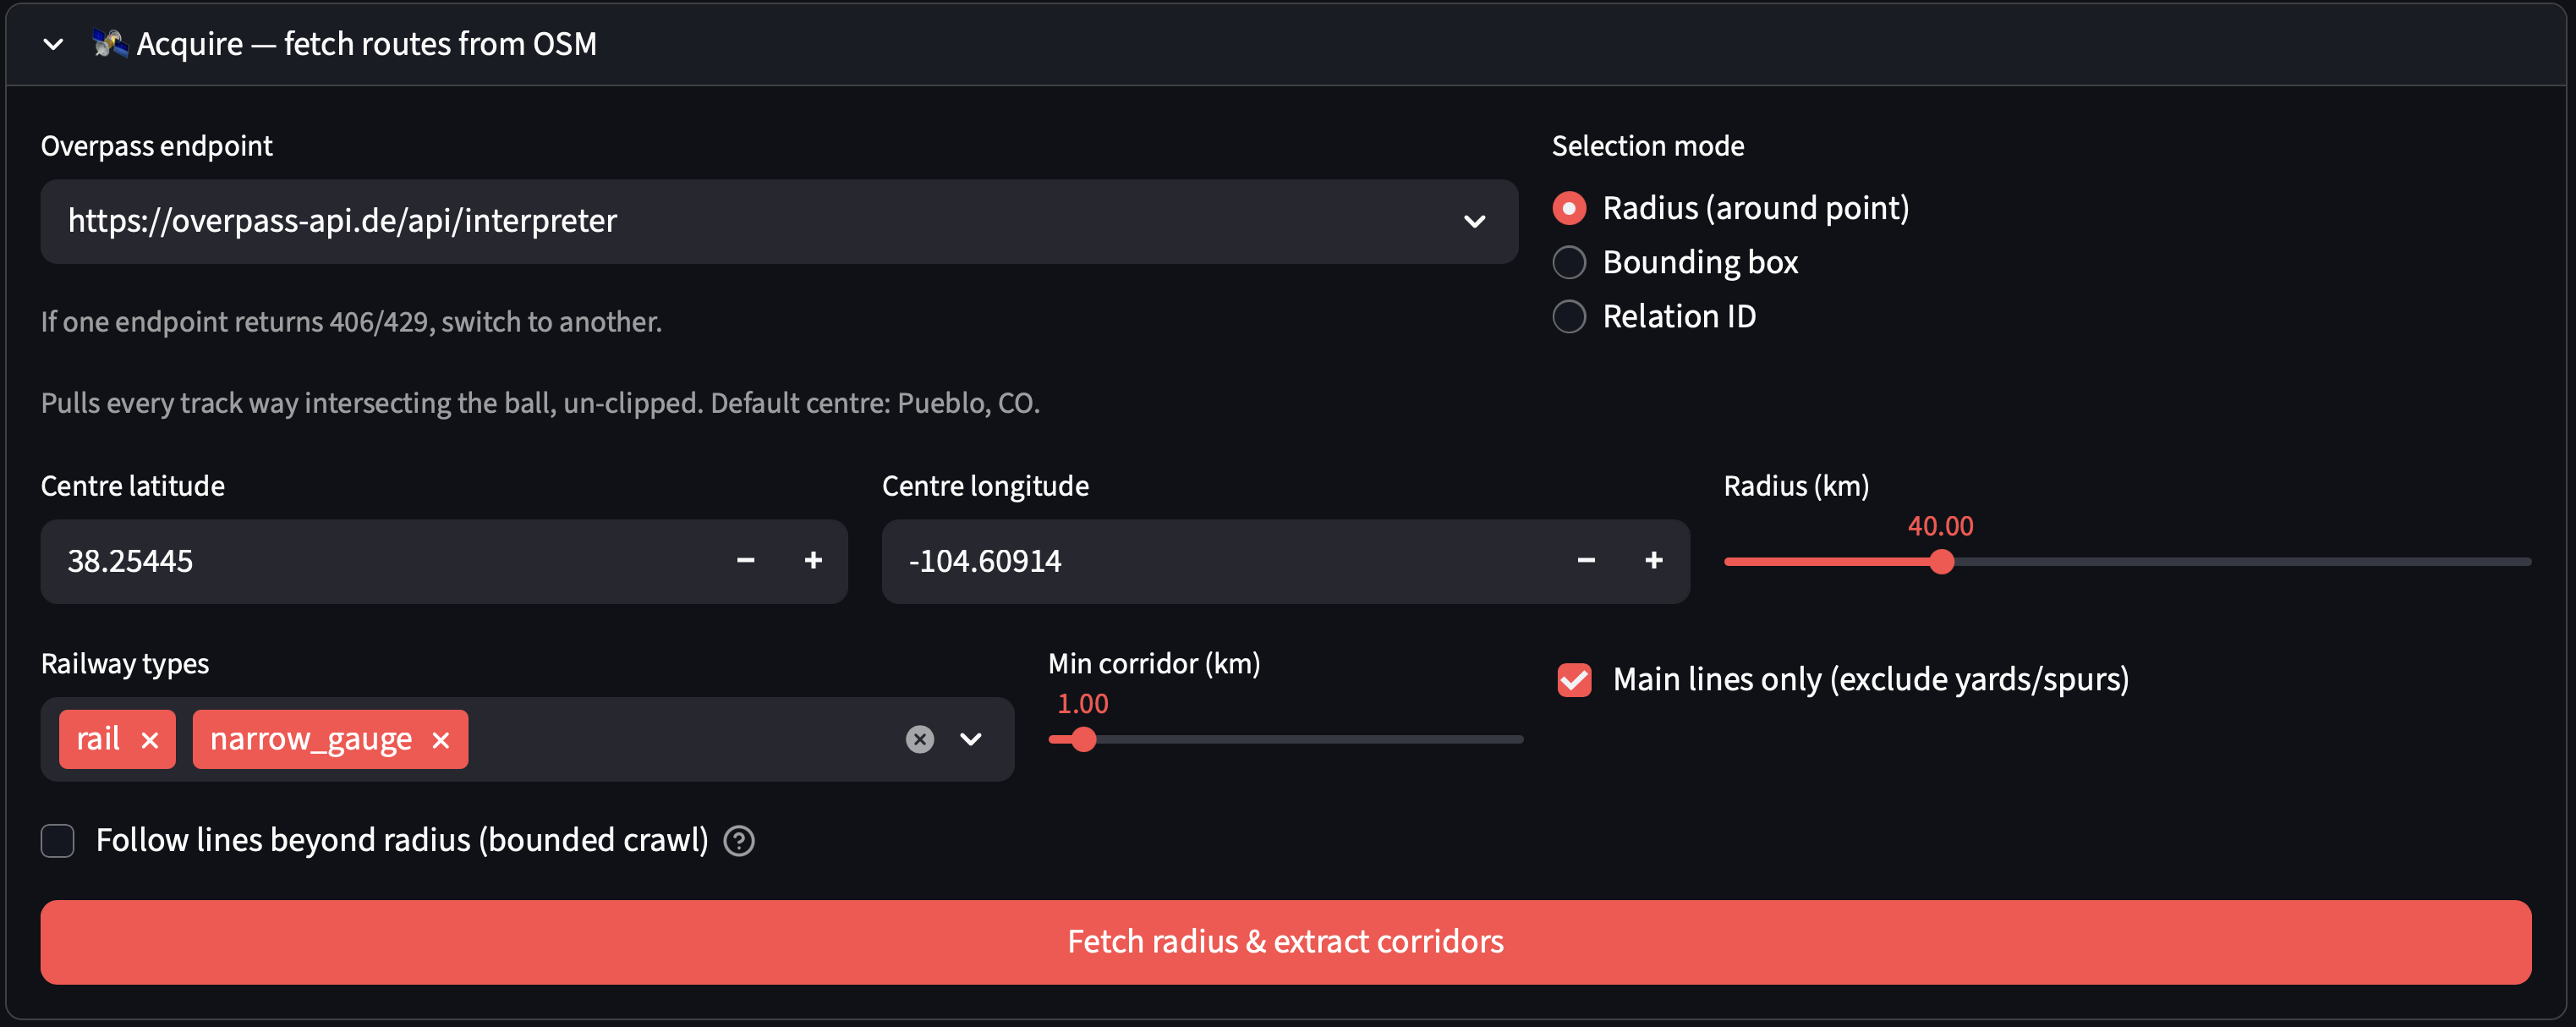
\includegraphics[width=0.92\textwidth]{thesis_imgs_7_15/route_generator/route_aq_page1.png}
    \caption{The acquisition panel of the route application. A selection mode (radius, bounding box, or relation identifier) is chosen on the right; the centre point, radius, admissible railway types, and a minimum corridor length are set on the left. The mainline-only filter excludes yards and spurs, and the bounded outward crawl described in \cref{sec:route_acquisition_stage1} is toggled at the bottom. Several Overpass endpoints are selectable because any one of them may be rate-limiting at a given moment.}
    \label{fig:route_acquire_panel}
\end{figure}

An accompanying Streamlit application exposes both acquisition modes. In area mode, a user enters a bounding box, the app fetches and extracts all corridors in it, and shows them color-coded on a map alongside a sortable table and per-corridor quality checks (gap count and size, branch points, how much of the line has known speed limits, and what fraction runs over bridges or through tunnels). Corridors selected from this view are added to a batch for export. In relation mode, a single named route is fetched and inspected the same way. For the common case of just wanting a handful of routes near a particular place, the simplest path is radius mode with the outward crawl enabled: a user clicks a line on the map, its full extent highlights, and it is written to storage with every vertex's structural flags and speed-limit coverage already attached.

\section{Stage 1.5: Resampling to a uniform grid}
\label{sec:route_resample}

OSM digitizes track adaptively with respect to horizontal curvature: dense vertices on curves, sparse vertices on straight tangents. That density pattern is a poor match for what the next stage needs, since it under-samples exactly the straight, low-curvature stretches where the vertical profile, grade, still needs to be captured accurately. The resampling stage rewrites each stored route onto a fixed arc-length grid (10 meter spacing by default) by linearly interpolating longitude and latitude along the line's arc length.

Two details matter here. First, step-valued features, speed limit, way identifier, and the bridge, tunnel, cutting, and embankment flags, are not smoothly interpolated; each resampled point simply inherits the value from whichever source segment it falls inside, and a sample is inserted exactly at the point where such a feature changes, so a speed-limit step or a bridge entrance is not blurred across a grid cell. Second, the resampling step validates its own output: coincident vertices are dropped, arc length is enforced to be strictly increasing, and each point is tagged with the length of the source segment it came from and a flag marking whether it was interpolated across an unusually long or bridged gap in the original data.

\begin{figure}[htbp]
    \centering
    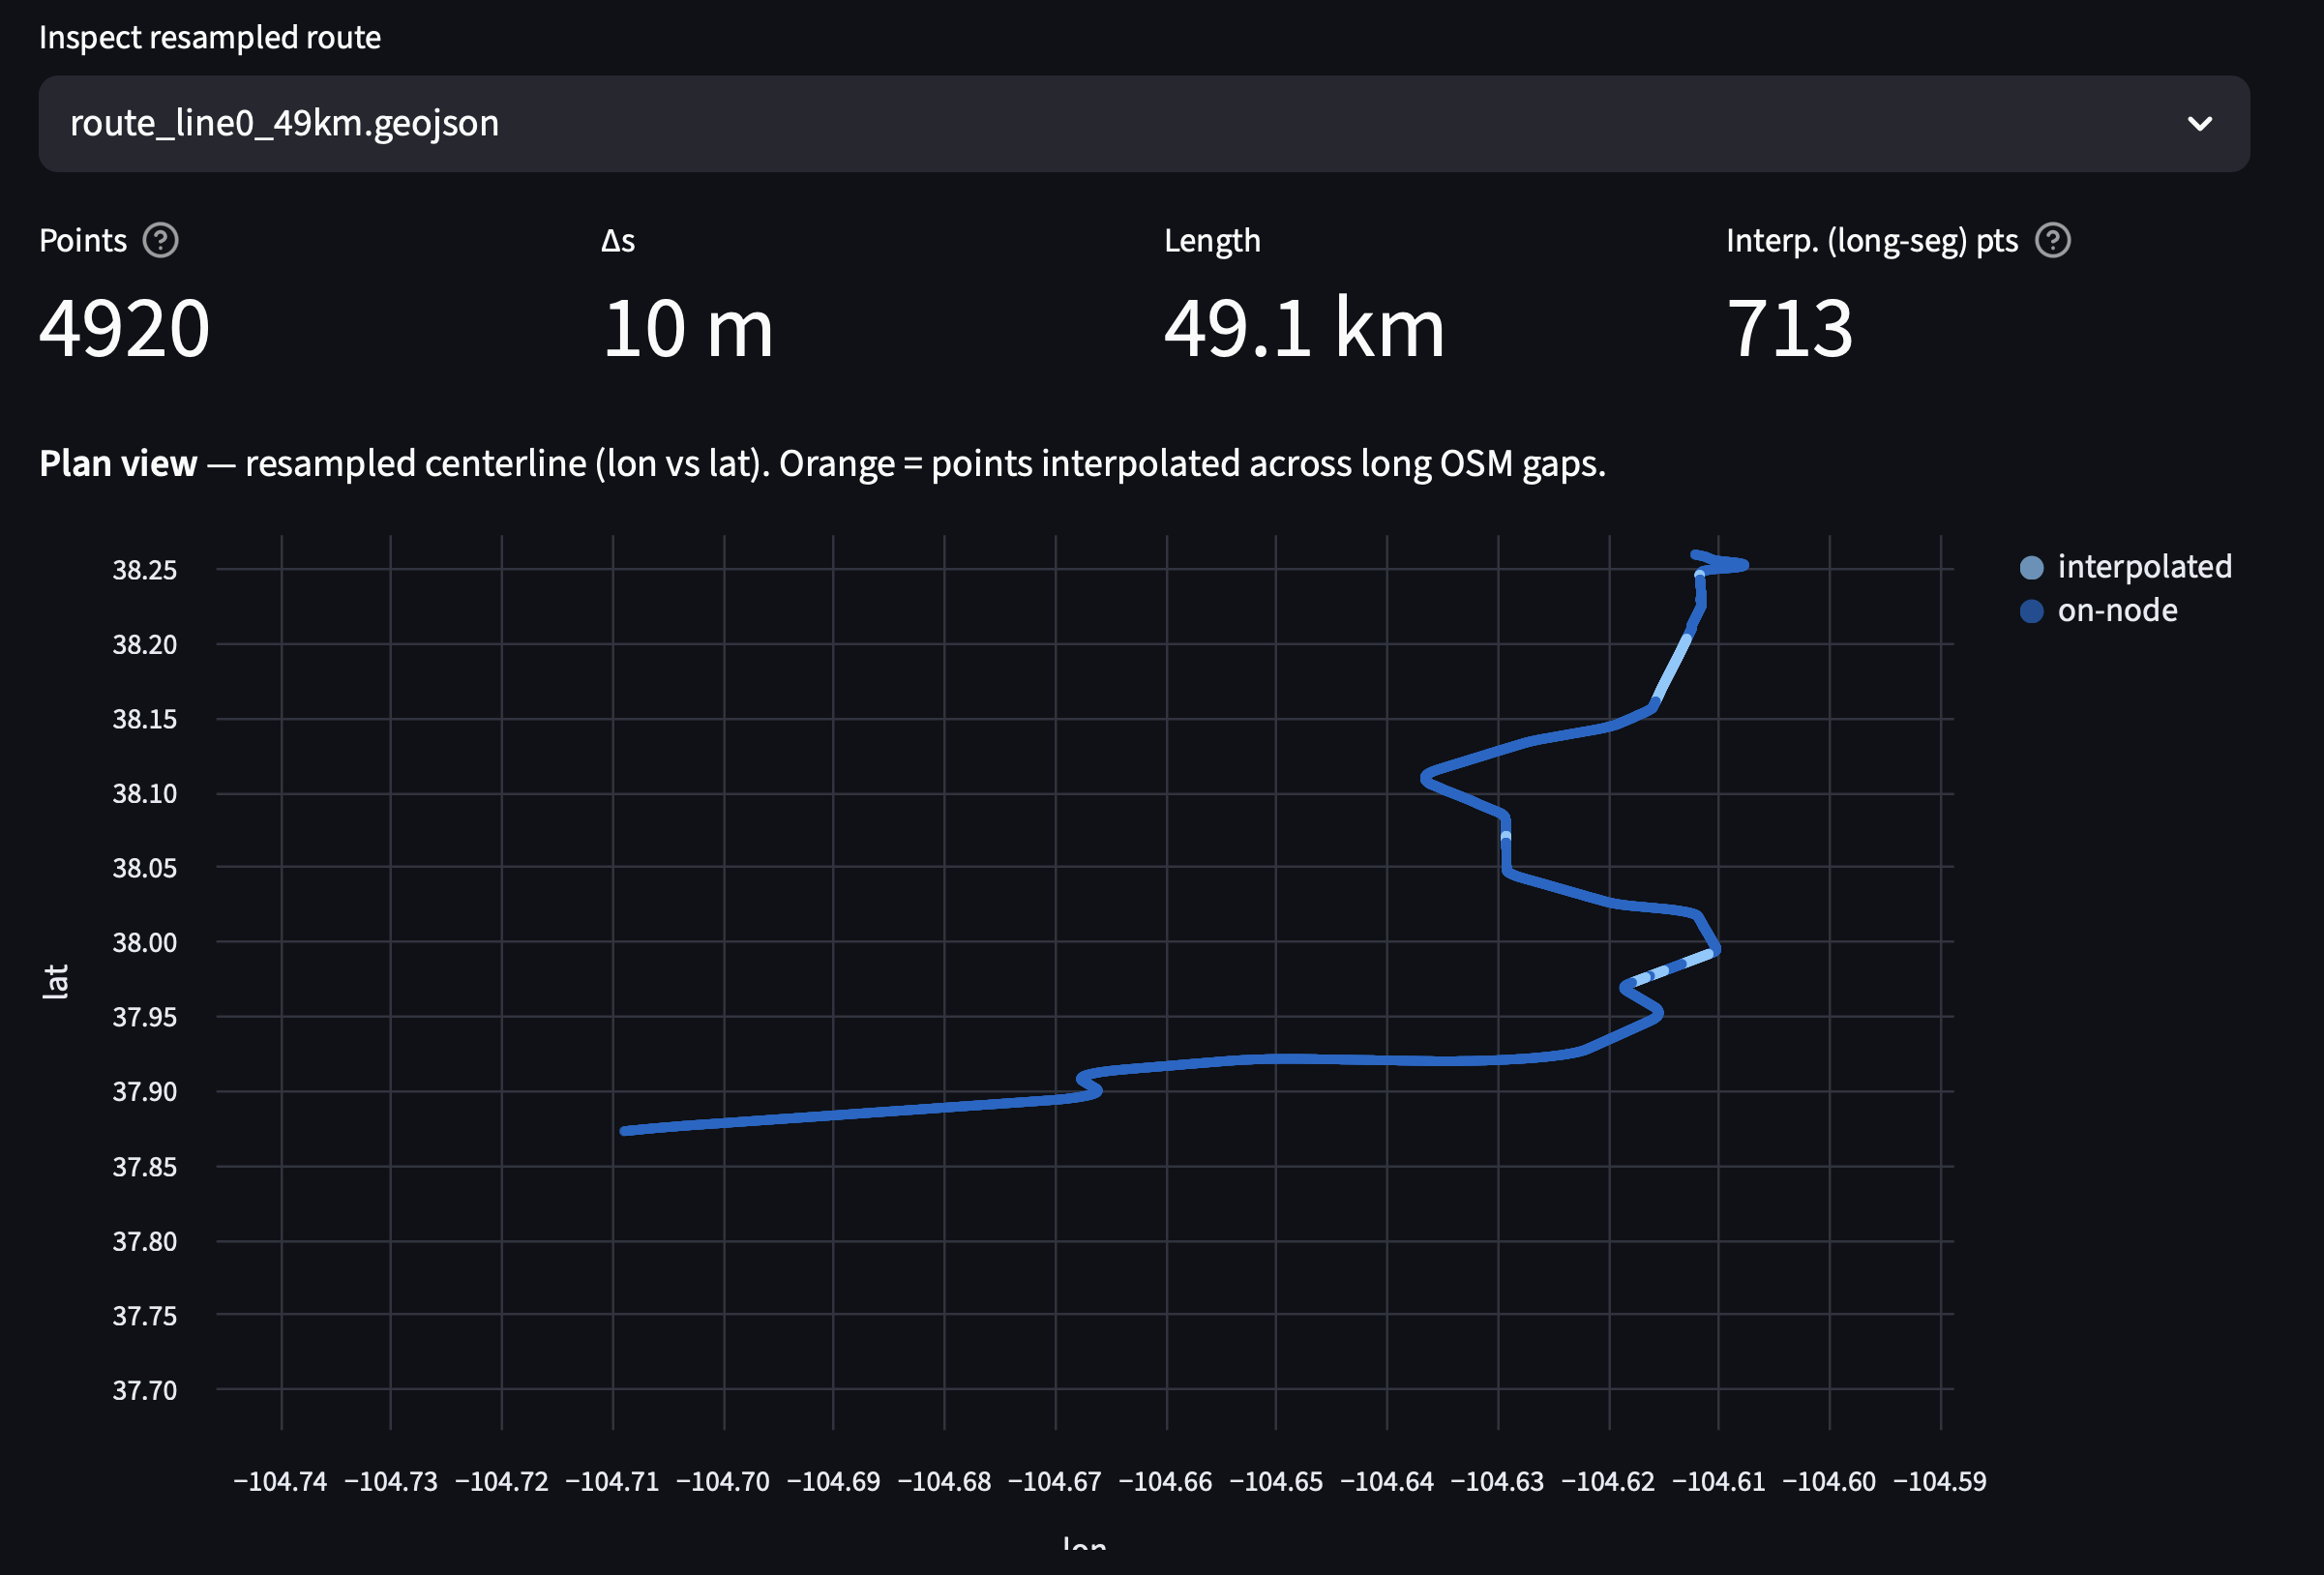
\includegraphics[width=0.92\textwidth]{thesis_imgs_7_15/route_generator/route_resample.png}
    \caption{Inspection view for a resampled route: a 49.1\,km corridor rewritten onto a uniform 10\,m grid, yielding 4920 points. The plan view distinguishes points that sit on an original map vertex from those interpolated across long source segments (713 of them here), so stretches where the geometry is inferred rather than mapped remain visible downstream.}
    \label{fig:route_resample}
\end{figure}

\section{Stage 2: Elevation}
\label{sec:route_elevation}

Each resampled point is next given a ground elevation from the USGS 3DEP digital elevation model (DEM) \cite{usgs3dep}, producing a three-dimensional route as a sequence of longitude, latitude, and elevation triples. Elevation is queried in batches against 3DEP's image-service endpoint, since it accepts many points per request, with a slower per-point service used as a fallback for any vertex the batch call cannot resolve. Batches hold 1000 points, the most the service returns in one response, and are sent as POST requests, since a request of that size is too long to carry in a URL. Up to sixteen batches run concurrently. Because each request is limited by network latency rather than by server work, throughput scales almost linearly with the number of concurrent requests, reaching about 16,000 points per second. A batch that fails is reported as a failure rather than silently passed to the per-point fallback, which would otherwise hide a broken batch path behind a pipeline that still works, only several hundred times more slowly. Requests retry with backoff when the service is busy or briefly unavailable. Any point elevation cannot be determined for is left as a missing value rather than guessed, and every earlier per-vertex field from acquisition and resampling is preserved alongside the new elevation data.

\begin{figure}[htbp]
    \centering
    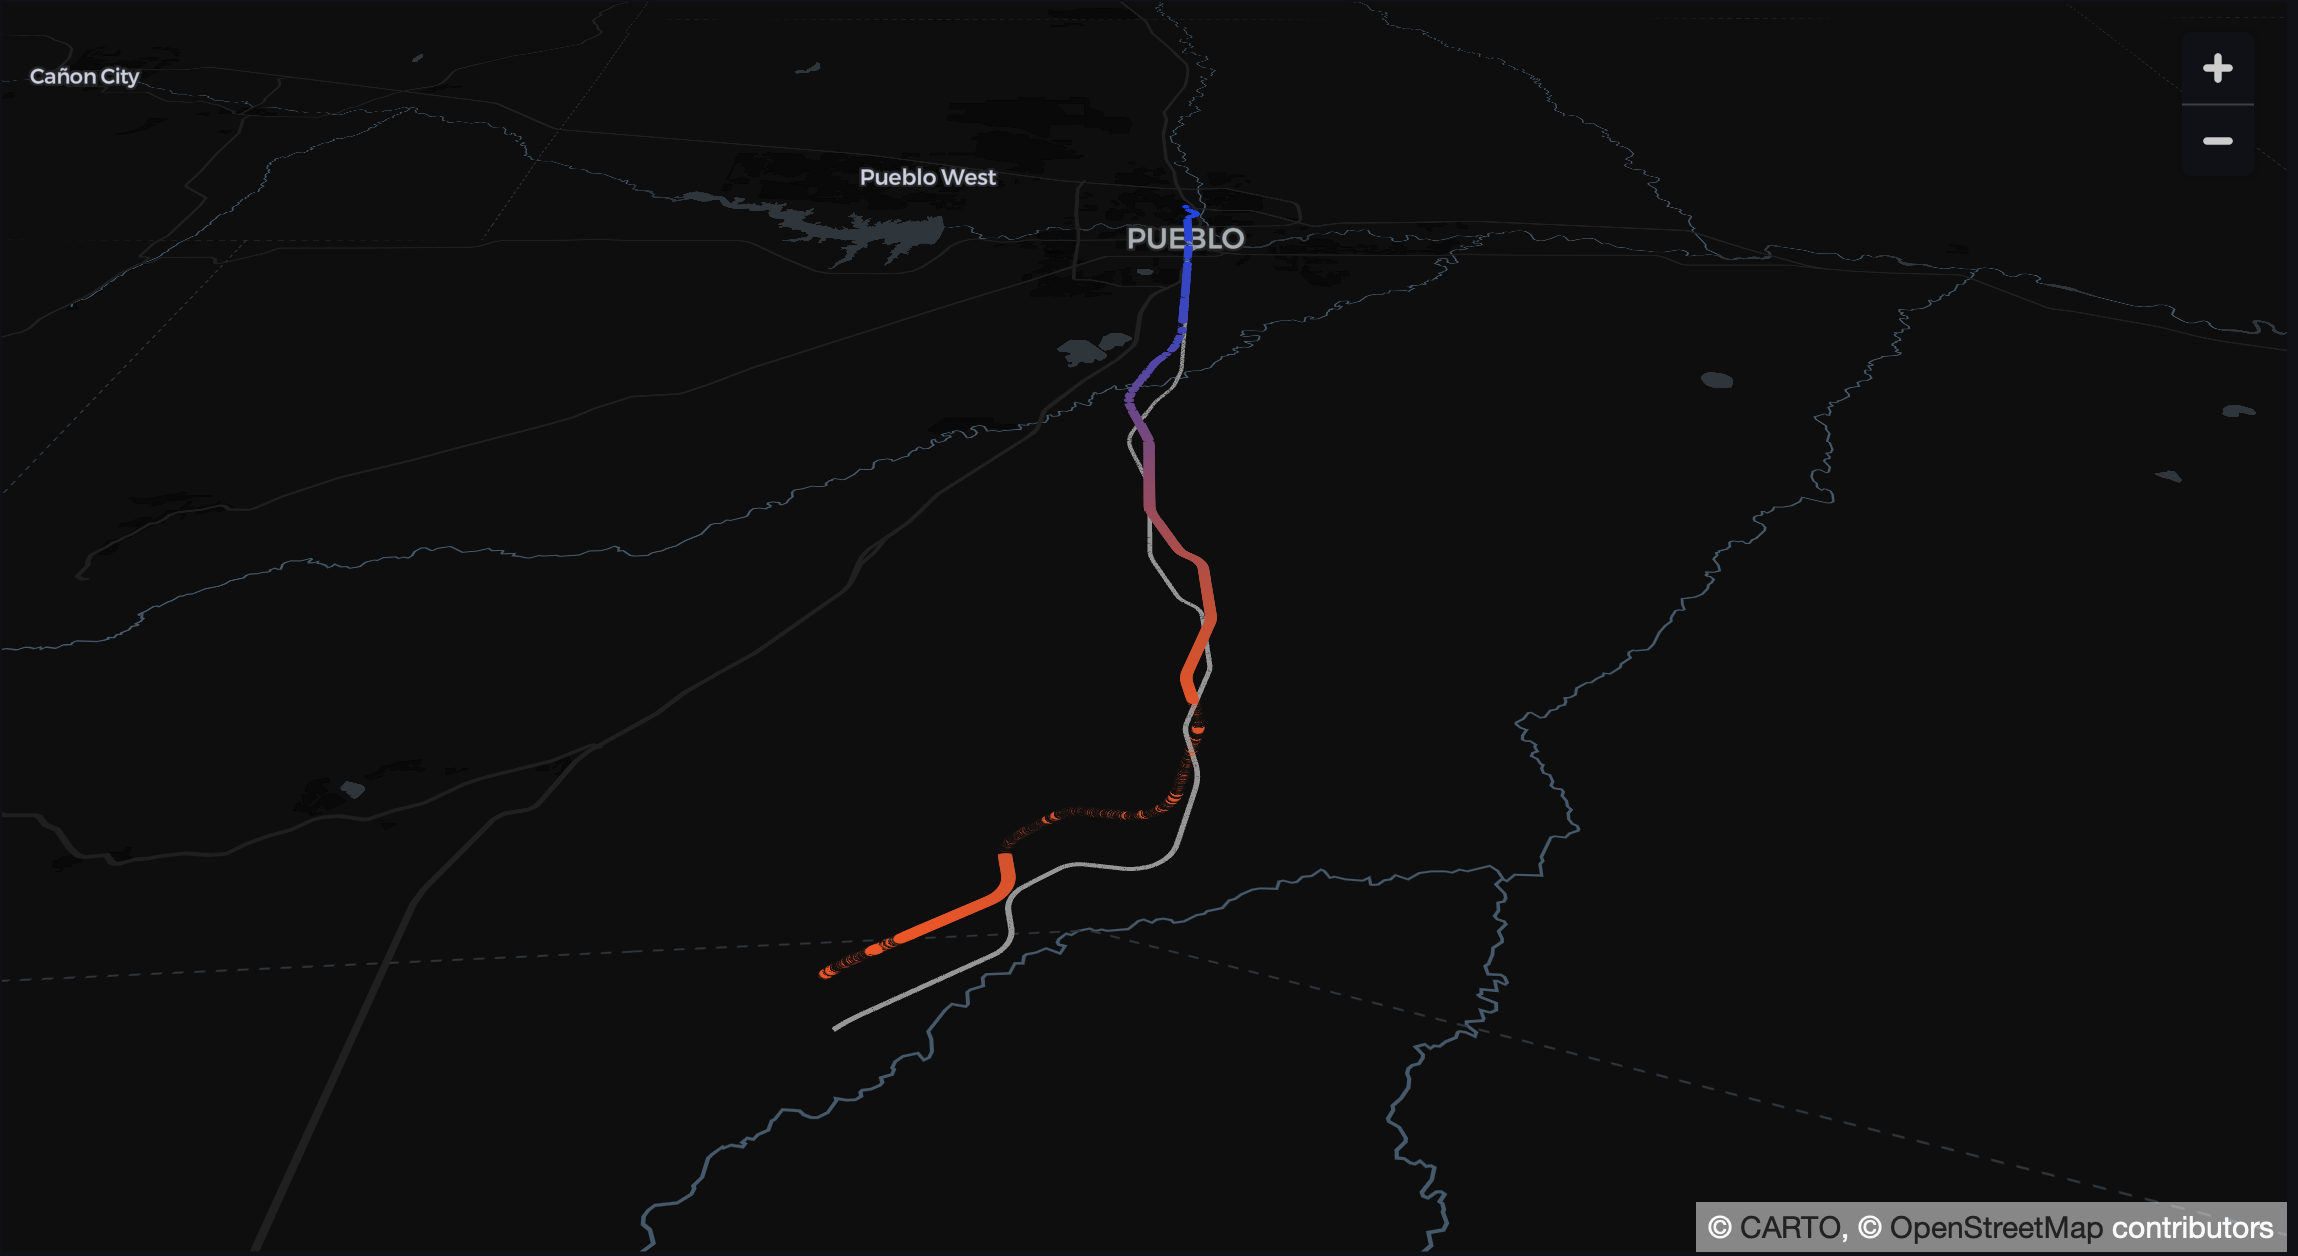
\includegraphics[width=0.92\textwidth]{thesis_imgs_7_15/route_generator/routes_elevated.png}
    \caption{An elevated route rendered in three dimensions, coloured by elevation along the line, with the mapped ground track shown alongside. Visual inspection at this stage catches corridors that have been stitched incorrectly or that jump between parallel alignments, before any derivative is taken.}
    \label{fig:route_elevated}
\end{figure}

\begin{figure}[htbp]
    \centering
    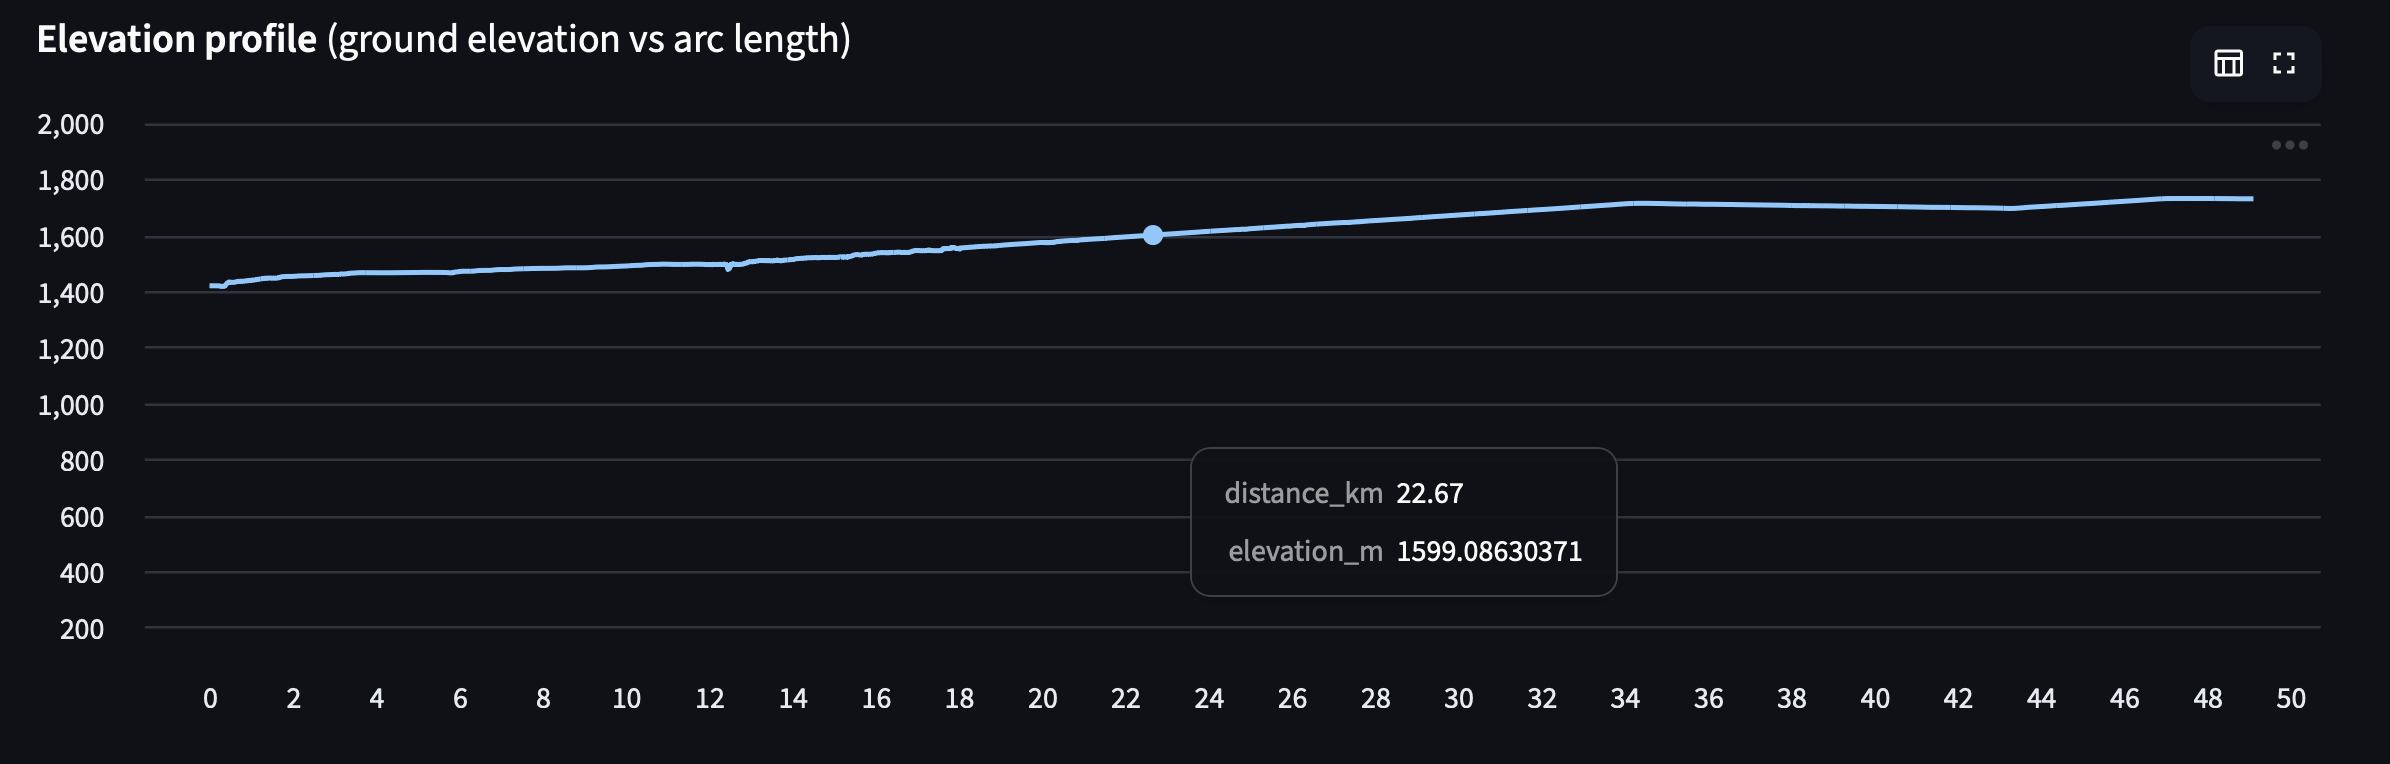
\includegraphics[width=0.92\textwidth]{thesis_imgs_7_15/route_generator/route_elevation_profile.png}
    \caption{Ground elevation against arc length for the same corridor, climbing from roughly 1430\,m to 1740\,m over 49\,km. This is the raw signal from which grade is derived; the metre-scale error it carries is negligible against the elevation range plotted here but is large against the elevation \emph{change} between adjacent 10\,m samples, which is what motivates the smoothing described below.}
    \label{fig:route_elevation_profile}
\end{figure}

\section{Checking the raw elevation}
\label{sec:route_raw_qa}

A grade field can be wrong in two ways. The elevation can be correct but too noisy for the chosen smoothing window, in which case a wider window fixes it. Or the elevation can be wrong at the source, because the samples do not lie on the track: the mapped centreline has drifted off the real alignment, or the elevation model does not resolve a cutting or embankment and reports the ground beside it. No smoothing window repairs the second case. Smoothing incorrect values only averages them, and widening the window far enough to hide the error also flattens the real terrain on every healthy corridor.

The two cases can be told apart before any smoothing is done, by looking at the raw elevation directly. \Cref{tab:route_raw_qa} gives three measures of raw roughness for the five corridors. The key one is the share of 10\,m steps whose elevation changes by more than a metre. A one-metre change over ten metres is a 10\% grade, far steeper than any freight main line, so a corridor where this happens on a large share of steps is not following the track.

\begin{table}[htbp]
    \centering
    \begin{tabular}{lccc}
        \toprule
        Corridor & Median $|\Delta z|$ per step & Steps with $|\Delta z| > 1$\,m & Second-difference roughness \\
        \midrule
        \texttt{route\_line0} & 0.077\,m & 0.7\% & 0.021\,m \\
        \texttt{route\_line2} & 0.234\,m & \textbf{19.3\%} & 0.143\,m \\
        \texttt{route\_line3} & 0.047\,m & 1.5\% & 0.040\,m \\
        \texttt{route\_line4} & 0.039\,m & 1.1\% & 0.036\,m \\
        \texttt{route\_line5} & 0.045\,m & 1.0\% & 0.041\,m \\
        \bottomrule
    \end{tabular}
    \caption{Roughness of the raw elevation, before any smoothing, for the five acquired corridors on a 10\,m grid. \texttt{route\_line2} exceeds a one-metre step on nearly a fifth of its length, against 0.7--1.5\% for the others. Its bridge and tunnel share is under 1\%, so structure correction does not explain the difference.}
    \label{tab:route_raw_qa}
\end{table}

The expected explanation for the poor grade field on \texttt{route\_line2}, an rms grade of 2.46\% against about 0.9\% elsewhere, was too little smoothing. The table shows that it was not. The raw elevation is already wrong before smoothing, and a search for a window wide enough to hide it settled on 1200\,m, a value that would have erased real terrain on the other four corridors to rescue one broken one.

The pipeline therefore checks the raw elevation first. A corridor on which more than 5\% of steps change by more than a metre is rejected, and the smoothing window is chosen only over the corridors that pass. \texttt{route\_line2} fails the check and is removed, leaving four corridors. The window is then set to the narrowest value, 800\,m, at which the grade limit stops binding on every remaining corridor.

The grade limit was lowered from 4\% to 2.5\% at the same time, and its role changed. A limit of 4\% is well above the grades freight main lines are built to, so it clipped the broken corridor's grade without drawing attention to it. At 2.5\%, reaching the limit is itself a sign of an error in the data, and the fraction of a corridor that reaches it is reported. \Cref{tab:route_grade_stats} gives the resulting grade statistics.

\begin{table}[htbp]
    \centering
    \begin{tabular}{lcccc}
        \toprule
        Corridor & rms grade & 95th percentile & Maximum & Share at limit \\
        \midrule
        \texttt{route\_line0} (49\,km) & 0.86\% & 1.45\% & 2.50\% & 1.0\% \\
        \texttt{route\_line3} (29\,km) & 0.72\% & 1.25\% & 1.47\% & 0.0\% \\
        \texttt{route\_line4} (27\,km) & 0.39\% & 0.75\% & 1.23\% & 0.0\% \\
        \texttt{route\_line5} (22\,km) & 0.58\% & 0.87\% & 1.17\% & 0.0\% \\
        \bottomrule
    \end{tabular}
    \caption{Grade statistics for the four corridors that pass the raw-elevation check, with an 800\,m smoothing window and a 2.5\% grade limit.}
    \label{tab:route_grade_stats}
\end{table}

\texttt{route\_line0} still reaches the limit on 1.0\% of its length, in short runs with a median length of 135\,m. A real ruling grade is held for kilometres, so these runs are residual artifacts rather than terrain. They fall within the tolerance, and a filter on the minimum length of a grade excursion would be a more physical fix than further smoothing.

The effect on simulated trains is direct. In scenarios run on the old grade field, the fastest overspeed reached 67.8\,m/s, a freight train travelling at about 245\,km/h, and these extreme cases came from the false grades of \texttt{route\_line2}. On the corrected corridors the worst case falls to 25.7\,m/s. The share of scenarios exceeding the speed limit by more than 5\,m/s does not change, which shows it has a separate cause. That cause lies in how driving commands are generated, not in the terrain, and it is discussed with the dataset.

The two datasets described in \cref{ch:gpu_dataset} were generated before this check existed, and both include \texttt{route\_line2}; \cref{sec:dataset_limitations} states what that means for results measured on them.

\section{Stage 3: Deriving the route profile}
\label{sec:route_profile_derivation}

This is the stage that produces the exact fields the reference simulator and the surrogate consume: the grade field $\sin\theta(s)$, the curvature proxy $\kappa(s)$, and the speed limit $v_{\max}(s)$ introduced in \cref{sec:input_definitions}.

\subsection{Correcting for bridges and tunnels}

On a bridge or inside a tunnel, the DEM reports the elevation of the structure or the ground above it, not the elevation of the rail itself, and it sometimes reports no value at all. These stretches are identified using the structural flags carried since acquisition, discarded, and filled in by linear interpolation across the gap.

\subsection{Smoothing and differentiating together}

Raw DEM elevation carries roughly a meter of error, which is small compared to elevation itself but large compared to elevation's rate of change. Differentiating the raw signal directly would produce a grade estimate that is almost entirely noise. Instead, a Savitzky-Golay filter \cite{savitzky1964smoothing} is applied, which fits a local polynomial through a moving window of points and yields a smoothed elevation value and its analytic derivative from the same operation, rather than smoothing and differentiating as two separate, error-compounding steps. Grade is then computed as $\sin\theta = \sin(\arctan(\mathrm{d}z/\mathrm{d}s))$, with a clamp on the maximum grade. The width of the smoothing window and the value of the clamp were both set by the corridor check described in \cref{sec:route_raw_qa}: an 800\,m window and a limit of 2.5\%.

Curvature is derived the same way. The horizontal coordinates are projected into a local planar frame, and the first and second Savitzky-Golay derivatives of that planar path give
\begin{equation}
    \kappa = \frac{x' y'' - y' x''}{\left(x'^2 + y'^2\right)^{3/2}},
    \label{eq:route_curvature}
\end{equation}
clamped to a minimum turning radius for the same reason grade is clamped.

\subsection{Speed limit and output}

Speed limit is converted from the map's tagged value into meters per second where available, and falls back to an estimate based on the Federal Railroad Administration's track classes \cite{fra_track_classes} where OSM coverage is missing. The finished profile is written in two forms: a GeoJSON file for visual inspection, and a compact array file holding exactly the fields \texttt{route\_s}, \texttt{route\_sin\_theta}, \texttt{route\_kappa}, and \texttt{route\_vmax}, matching the route-tensor layout used for dataset generation (\cref{ch:refsim}). As a final check, the array file is used to construct an actual route-profile object and sample it, confirming the file behaves correctly before it is trusted for later stages.

\begin{figure}[htbp]
    \centering
    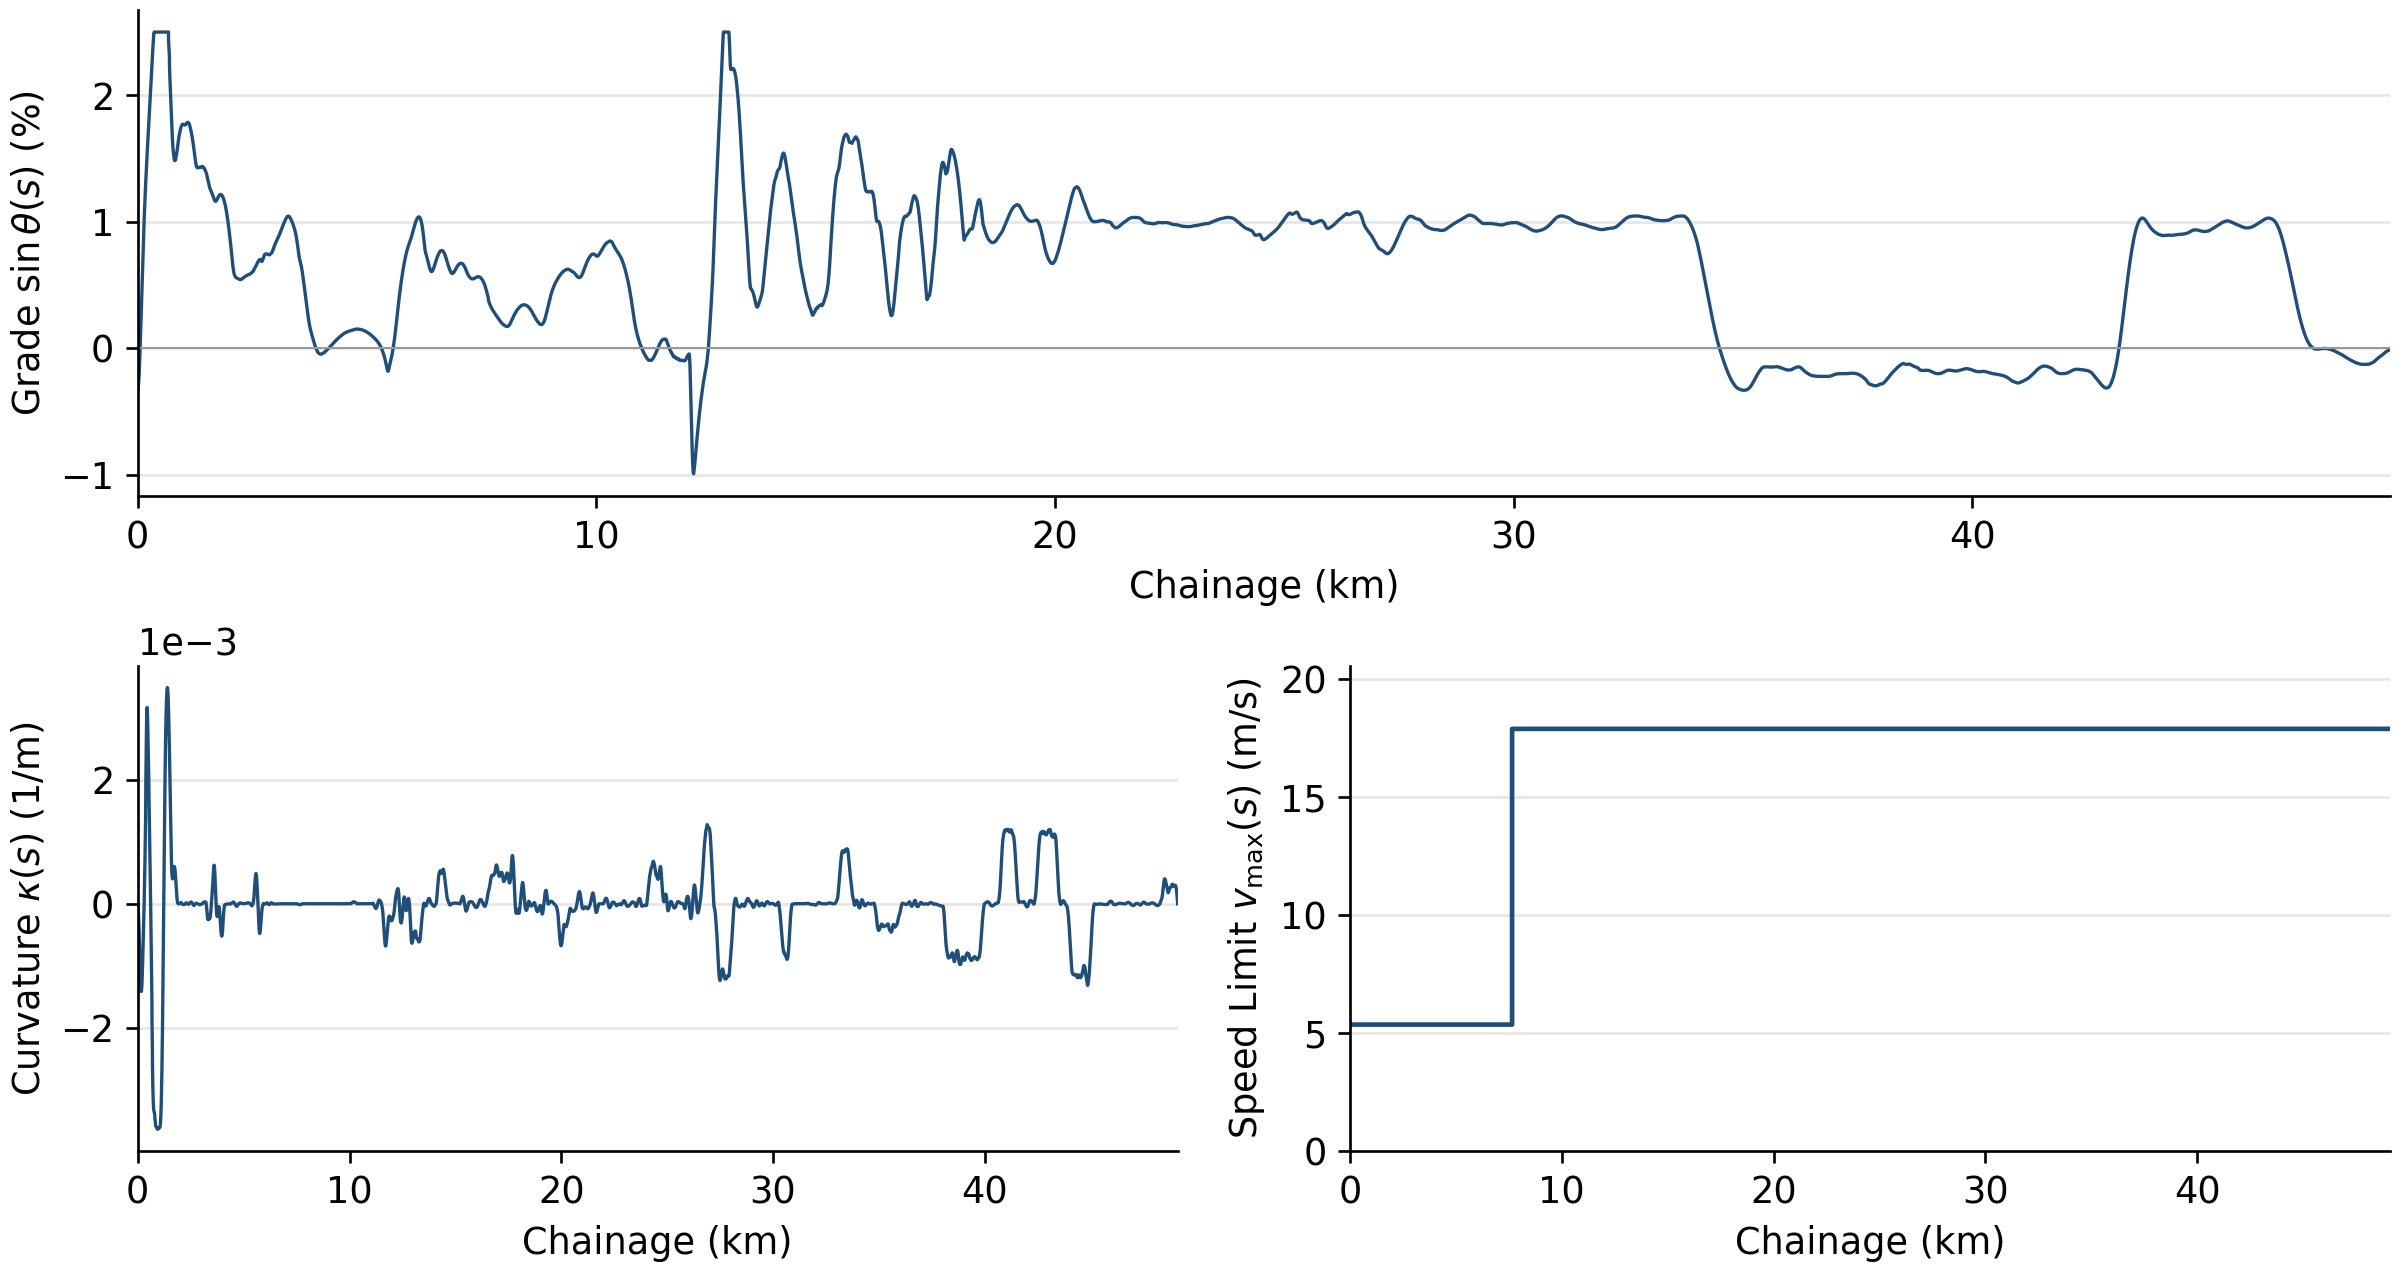
\includegraphics[width=0.92\textwidth]{thesis_imgs_7_15/route_generator/route_grade_curvature.png}
    \caption{The three derived fields the simulator consumes for \texttt{route\_line0}, plotted against chainage in kilometres: grade $\sin\theta(s)$ as a percentage (top), the curvature proxy $\kappa(s)$ (bottom left), and the speed limit $v_{\max}(s)$ (bottom right). Fields are shown after the corridor check of \cref{sec:route_raw_qa}, with an 800\,m smoothing window and a 2.5\% grade limit. The noisier grade over the first 20\,km is the urban approach, where frequent bridges, junctions, and short mapped segments degrade the elevation signal; beyond it the line settles onto a sustained climb near one percent. The grade reaches the 2.5\% limit only in two short runs, near the start and near 12.7\,km, which are residual artifacts rather than terrain. The speed limit is a step field, here rising where the line leaves restricted urban trackage.}
    \label{fig:route_grade_curvature}
\end{figure}

\section{Export}
\label{sec:route_export}

Finished routes are collected into a single export bundle: one array file per route, an index summarizing each route's location, endpoints, length, and grade and curvature statistics, and a manifest recording what each channel means and how the route was produced. This bundle is the handoff point between route acquisition and dataset generation; its array files drop directly onto the reference simulator's route-profile input with no further conversion.

\section{Scaling beyond a handful of corridors}
\label{sec:route_scaling}

Five corridors are enough to build and test the pipeline, but not enough to support a strong claim about generalization to unseen routes, or to hold out a genuinely steep corridor for evaluation. The next step was therefore a larger, regional corridor set, and the pipeline was extended for it.

\subsection{The batch crawl}

For more than a few routes, a headless batch runner replaces the interactive application. It takes a curated list of seed points, runs the area-first acquisition and bounded outward crawl of \cref{sec:route_acquisition_stage1} from each, and merges the results into one dataset. Lines pulled from overlapping seeds are deduplicated by their shared map identifiers, keeping the longest version of any line pulled more than once, and the run caches each seed so it can resume after an interruption. Several measures keep individual queries to the Overpass service from timing out: service track and industrial, tourism, and military spurs are excluded at query time, the initial query for each seed is split into a grid of small requests, and every request retries with exponential backoff and can rotate across mirror servers.

A regional run of 22 seeds within 900\,km of Pueblo, Colorado, chosen to include steep crossings such as Raton Pass and Tennessee Pass, did not complete. It failed on five consecutive seeds with server-busy errors over 4.5 hours. The choice of server had been based on the time to answer a single test query, and a single query does not predict a sustained crawl: a server that answers one request quickly may throttle heavily once hundreds arrive. Retries and backoff do not help when the limit is the server's tolerance for the workload itself.

\subsection{The North American Rail Network}

The crawl was replaced by a different source of track geometry. The U.S. Department of Transportation's Bureau of Transportation Statistics publishes the North American Rail Network, a national dataset of rail line segments covering the United States, Canada, and Mexico, as a queryable feature service \cite{narn}. It removes the two hardest parts of the OSM path.

\begin{itemize}
    \item \textbf{Topology is explicit.} Every segment records the node it starts from and the node it ends at, so the network is already a graph. The OSM path had to reconstruct connectivity from fragment endpoints, which is where its gaps and branch-ordering problems came from.
    \item \textbf{Track is already classified.} Each of the 302,771 segments carries a network class assigned by the data's maintainers. Main-line track accounts for 95,936 segments; the rest are yard tracks, industrial leads, passing sidings, and out-of-service or abandoned line. The mainline filter that the OSM path approximated with tag rules is given directly.
\end{itemize}

It also carries attributes OSM did not reliably provide, including the owning railroad, the subdivision name, and the number of tracks, so corridors can be identified by their real names rather than by labels such as \texttt{route\_line2}. No rate limiting was observed. The full main-line network, 95,936 segments and 274,145\,km of track, was downloaded in 13.5 minutes.

The network does not include line speeds, so speed limits still come from OSM, queried per corridor rather than crawled. Elevation still comes from 3DEP. With the batched elevation queries of \cref{sec:route_elevation}, the rest of the pipeline is fast enough for the whole network: resampling, elevation, and profile derivation for all 274,145\,km at 10\,m spacing, about 27 million points, are projected to take roughly 36 minutes, almost all of it in elevation queries.

\subsection{What remains}

The network is a graph of segments averaging 2.9\,km in length, not a set of routes. The simulator needs continuous corridors with a single, increasing chainage, so one stage is still missing before resampling: traversing the graph into corridors. Railroad subdivisions are the natural unit, since they are how railroads divide their own networks, and the dataset names 2,492 of them. How to order segments within a subdivision, and how to handle subdivisions that branch, are open questions. This stage has not been implemented, and the datasets used in this thesis are built on the OSM corridors described earlier in the chapter.

\section{Testing and design choices}
\label{sec:route_design}

The line-stitching logic, the part of the pipeline responsible for turning disordered, possibly reversed map fragments into one correct ordered corridor, is unit tested offline against a fixture built from a captured query response, so its correctness does not depend on network access or on live map data staying unchanged.

A few choices run through the whole pipeline. Acquisition and assembly are pure functions wherever they do not require a live network call, which is what makes offline testing possible in the first place. Data quality problems are surfaced rather than silently patched: gaps are bridged but their size is reported, branch points are flagged rather than resolved automatically, and disconnected fragments are dropped and listed rather than dropped quietly, so a user decides whether a given route is clean enough to use. Finally, the core pipeline, acquisition, resampling, elevation fusion, and profile derivation, depends only on NumPy and an HTTP request library; the Savitzky-Golay smoothing and differentiation is a small NumPy implementation of its own rather than a dependency on a larger scientific computing package, so the whole path can run and be tested without a heavier install.

\section{Chapter summary}

This chapter documented the pipeline that turns raw OpenStreetMap track data and public elevation data into the route profiles this thesis relies on: area-based acquisition and graph-based corridor extraction, fragment stitching back into whole lines, resampling onto a uniform grid, elevation fusion, a check on the raw elevation, and Savitzky-Golay-based derivation of grade, curvature, and speed limit. The raw-elevation check rejected one of the five acquired corridors, whose elevation samples did not lie on the track, and set the smoothing window and grade limit over the four that remain. For a larger corridor set, the OSM crawl was replaced by the North American Rail Network, which supplies explicit topology and track classification for the whole continent; converting that network into corridors is the remaining step. The output, arrays of \texttt{route\_s}, \texttt{route\_sin\_theta}, \texttt{route\_kappa}, and \texttt{route\_vmax}, is exactly what the reference simulator in \cref{ch:refsim} consumes and what later chapters use to generate training data for the surrogate. Because this pipeline draws on real corridors rather than invented ones, it is also what makes it possible to hold out whole real corridors for the generalization experiments described in later chapters, rather than only holding out synthetic variations of the same underlying route.
